% =====================================================================
%  KHÓA LUẬN TỐT NGHIỆP — UIT (ĐHQG-HCM)
%  Đề tài: Dự báo suy giảm tài chính doanh nghiệp bán lẻ từ dữ liệu SEC XBRL
%  Biên dịch: XeLaTeX (khuyến nghị). Chạy: xelatex -> bibtex -> xelatex x2
%  Quy chuẩn: Phụ lục 2 (hình thức trình bày) & Phụ lục 3 (mẫu báo cáo)
% =====================================================================
\documentclass[13pt,a4paper]{extreport}

% ---------- Ngôn ngữ & font ----------
\usepackage{fontspec}
\setmainfont{Times New Roman}
\usepackage[vietnamese]{babel}
\usepackage{amsmath,amssymb}

% ---------- Khổ giấy & căn lề (Phụ lục 2) ----------
\usepackage[a4paper,top=3.0cm,bottom=3.5cm,left=3.5cm,right=2.0cm]{geometry}

% ---------- Dãn dòng 1.5 ----------
\usepackage{setspace}
\onehalfspacing

% ---------- Hình, bảng, chú thích ----------
\usepackage{graphicx}
\usepackage{float}
\usepackage{booktabs}
\usepackage{array}
\usepackage{longtable}
\usepackage{tabularx}
\usepackage{multirow}
\usepackage[font=small,labelfont=bf,justification=centering]{caption}

% ---------- Đánh số đến cấp 4 ----------
\setcounter{secnumdepth}{4}
\setcounter{tocdepth}{4}

% ---------- Định dạng tiêu đề (Phụ lục 2) ----------
\usepackage{titlesec}
\titleformat{\chapter}[display]
  {\normalfont\bfseries\centering\fontsize{14}{17}\selectfont}
  {\MakeUppercase{\chaptername}\ \thechapter}{0.4em}{\MakeUppercase}
\titlespacing*{\chapter}{0pt}{-10pt}{18pt}
\titleformat{\section}{\normalfont\bfseries\fontsize{13}{16}\selectfont}
  {\thesection}{0.6em}{}
\titlespacing*{\section}{0pt}{12pt}{6pt}
\titleformat{\subsection}{\normalfont\bfseries\fontsize{13}{16}\selectfont}
  {\thesubsection}{0.6em}{}
\titlespacing*{\subsection}{0pt}{10pt}{4pt}
\titleformat{\subsubsection}{\normalfont\bfseries\fontsize{13}{16}\selectfont}
  {\thesubsubsection}{0.6em}{}
\titlespacing*{\subsubsection}{0pt}{8pt}{4pt}
\titleformat{\paragraph}[runin]{\normalfont\bfseries}{\theparagraph}{0.6em}{}
\titlespacing*{\paragraph}{0pt}{6pt}{0.5em}

% ---------- Thụt đầu dòng mọi đoạn ----------
\usepackage{indentfirst}
\setlength{\parindent}{1.0cm}
\setlength{\parskip}{4pt}

% ---------- Danh sách ----------
\usepackage{enumitem}
\setlist{nosep,leftmargin=1.2cm}

% ---------- Đánh số trang: giữa-dưới ----------
\usepackage{fancyhdr}
\pagestyle{fancy}
\fancyhf{}
\cfoot{\thepage}
\renewcommand{\headrulewidth}{0pt}
\renewcommand{\footrulewidth}{0pt}

% ---------- Liên kết ----------
\usepackage[hidelinks,unicode]{hyperref}
\hypersetup{pdftitle={Du bao suy giam tai chinh doanh nghiep ban le tu du lieu SEC XBRL}}

% ---------- Code listing (Phụ lục) ----------
\usepackage{listings}
\usepackage{xcolor}
\lstset{
  basicstyle=\ttfamily\small,
  breaklines=true,
  frame=single,
  numbers=left,
  numberstyle=\tiny,
  keywordstyle=\color{blue!70!black},
  commentstyle=\color{green!40!black},
  showstringspaces=false,
  columns=flexible,
  keepspaces=true
}

% ---------- Nhãn tiếng Việt ----------
\renewcommand{\contentsname}{MỤC LỤC}
\renewcommand{\listfigurename}{DANH MỤC HÌNH VẼ}
\renewcommand{\listtablename}{DANH MỤC BẢNG BIỂU}
\renewcommand{\figurename}{Hình}
\renewcommand{\tablename}{Bảng}
\renewcommand{\bibname}{TÀI LIỆU THAM KHẢO}

\begin{document}

% =====================================================================
%  TRANG BÌA CHÍNH  (không hiển thị số trang)
% =====================================================================
\pagenumbering{gobble}
\begin{titlepage}
\centering
{\bfseries\fontsize{14}{17}\selectfont ĐẠI HỌC QUỐC GIA TP. HỒ CHÍ MINH\par}
\vspace{4pt}
{\bfseries\fontsize{16}{19}\selectfont TRƯỜNG ĐẠI HỌC CÔNG NGHỆ THÔNG TIN\par}
\vspace{10pt}
{\bfseries\fontsize{14}{17}\selectfont KHOA HỆ THỐNG THÔNG TIN\par}
\vspace{1.8cm}
{\bfseries\fontsize{14}{17}\selectfont <TÊN SINH VIÊN>\par}
\vspace{1.2cm}
{\bfseries\fontsize{16}{19}\selectfont KHÓA LUẬN TỐT NGHIỆP\par}
\vspace{1.0cm}
{\bfseries\fontsize{20}{24}\selectfont DỰ BÁO SUY GIẢM TÀI CHÍNH DOANH NGHIỆP\\[2pt] BÁN LẺ TỪ DỮ LIỆU SEC XBRL\\[2pt] BẰNG HỌC MÁY\par}
\vspace{0.6cm}
{\bfseries\fontsize{15}{18}\selectfont PREDICTING RETAIL FINANCIAL DISTRESS FROM SEC XBRL DATA USING MACHINE LEARNING\par}
\vfill
{\bfseries\fontsize{14}{17}\selectfont KỸ SƯ / CỬ NHÂN NGÀNH HỆ THỐNG THÔNG TIN\par}
\vspace{1.0cm}
{\bfseries\fontsize{13}{16}\selectfont TP. HỒ CHÍ MINH, <NĂM>\par}
\end{titlepage}

% =====================================================================
%  TRANG BÌA PHỤ
% =====================================================================
\begin{titlepage}
\centering
{\bfseries\fontsize{14}{17}\selectfont ĐẠI HỌC QUỐC GIA TP. HỒ CHÍ MINH\par}
\vspace{4pt}
{\bfseries\fontsize{16}{19}\selectfont TRƯỜNG ĐẠI HỌC CÔNG NGHỆ THÔNG TIN\par}
\vspace{10pt}
{\bfseries\fontsize{14}{17}\selectfont KHOA HỆ THỐNG THÔNG TIN\par}
\vspace{1.4cm}
{\bfseries\fontsize{14}{17}\selectfont <TÊN SINH VIÊN> -- <MÃ SINH VIÊN>\par}
\vspace{1.0cm}
{\bfseries\fontsize{16}{19}\selectfont KHÓA LUẬN TỐT NGHIỆP\par}
\vspace{0.8cm}
{\bfseries\fontsize{18}{22}\selectfont DỰ BÁO SUY GIẢM TÀI CHÍNH DOANH NGHIỆP\\[2pt] BÁN LẺ TỪ DỮ LIỆU SEC XBRL\\[2pt] BẰNG HỌC MÁY\par}
\vspace{0.5cm}
{\bfseries\fontsize{15}{18}\selectfont PREDICTING RETAIL FINANCIAL DISTRESS FROM SEC XBRL DATA USING MACHINE LEARNING\par}
\vspace{0.8cm}
{\bfseries\fontsize{14}{17}\selectfont KỸ SƯ / CỬ NHÂN NGÀNH HỆ THỐNG THÔNG TIN\par}
\vfill
\fbox{\parbox{11.5cm}{\centering
{\bfseries\fontsize{13}{16}\selectfont GIẢNG VIÊN HƯỚNG DẪN\par}
\vspace{0.8cm}
{\bfseries\fontsize{13}{16}\selectfont <TÊN GIẢNG VIÊN HƯỚNG DẪN>\par}}}
\vspace{0.8cm}
{\bfseries\fontsize{13}{16}\selectfont TP. HỒ CHÍ MINH, <NĂM>\par}
\end{titlepage}

% =====================================================================
%  THÔNG TIN HỘI ĐỒNG CHẤM KHÓA LUẬN
% =====================================================================
\chapter*{THÔNG TIN HỘI ĐỒNG CHẤM KHÓA LUẬN TỐT NGHIỆP}
\addcontentsline{toc}{chapter}{Thông tin hội đồng chấm khóa luận tốt nghiệp}
Hội đồng chấm khóa luận tốt nghiệp, thành lập theo Quyết định số ............ ngày ............. của
Hiệu trưởng Trường Đại học Công nghệ Thông tin.
\vspace{0.4cm}

\noindent\begin{tabularx}{\textwidth}{|>{\bfseries}p{6.4cm}|X|}
\hline
Thành phần hội đồng & Họ và tên \\
\hline
Chủ tịch hội đồng & .................................................... \\
\hline
Thư ký & .................................................... \\
\hline
Ủy viên 1 & .................................................... \\
\hline
Ủy viên 2 & .................................................... \\
\hline
Cán bộ phản biện & .................................................... \\
\hline
\end{tabularx}
\vspace{0.3cm}

\noindent Kết quả bảo vệ: ......................................... Điểm: ..................
\clearpage

% =====================================================================
%  LỜI CẢM ƠN
% =====================================================================
\chapter*{LỜI CẢM ƠN}
\addcontentsline{toc}{chapter}{Lời cảm ơn}
Nhóm chúng em xin cảm ơn giảng viên hướng dẫn đã định hướng đề tài và đặc biệt là yêu cầu kiểm
chứng dữ liệu về tận nguồn công bố thay vì tin vào kết quả in ra — yêu cầu đó định hình toàn bộ
cách làm của khóa luận. Chúng em cảm ơn quý thầy cô Khoa Hệ thống Thông tin đã trang bị nền tảng
về khai phá dữ liệu, học máy và đánh giá mô hình. Cảm ơn các bạn trong lớp đã phản biện và chỉ ra
những điểm số chưa hợp lý trong các bản báo cáo trước. Khóa luận còn nhiều hạn chế, nhóm mong nhận
được góp ý của hội đồng.
\clearpage

% =====================================================================
%  MỤC LỤC
% =====================================================================
\phantomsection
\tableofcontents
\clearpage

% =====================================================================
%  DANH MỤC HÌNH VẼ
% =====================================================================
\phantomsection
\addcontentsline{toc}{chapter}{Danh mục hình vẽ}
\listoffigures
\clearpage

% =====================================================================
%  DANH MỤC BẢNG BIỂU
% =====================================================================
\phantomsection
\addcontentsline{toc}{chapter}{Danh mục bảng biểu}
\listoftables
\clearpage

% =====================================================================
%  DANH MỤC TỪ VIẾT TẮT
% =====================================================================
\chapter*{DANH MỤC TỪ VIẾT TẮT}
\addcontentsline{toc}{chapter}{Danh mục từ viết tắt}
\noindent\begin{longtable}{>{\bfseries}p{3.6cm}p{10.6cm}}
10-K / 10-Q & Báo cáo thường niên / báo cáo quý nộp cho SEC \\
8-K & Báo cáo sự kiện bất thường nộp cho SEC \\
AP & Average Precision (diện tích dưới đường Precision--Recall) \\
AUROC & Diện tích dưới đường cong ROC \\
CI & Confidence Interval (khoảng tin cậy) \\
CV & Cross-Validation (kiểm định chéo) \\
EDA & Exploratory Data Analysis (phân tích khám phá dữ liệu) \\
FN / FP & False Negative (bỏ sót) / False Positive (báo động giả) \\
GroupKFold & Kiểm định chéo chia nhóm theo thực thể \\
HGB & HistGradientBoostingClassifier (scikit-learn) \\
IR & Imbalance Ratio (tỉ lệ lớp đa số chia lớp thiểu số) \\
LOCO & Leave-One-Company-Out \\
MCC & Matthews Correlation Coefficient \\
MD\&A & Management Discussion \& Analysis \\
MLP & Multi-Layer Perceptron (mạng nơ-ron nhiều lớp) \\
OOF & Out-of-fold (dự đoán ngoài fold) \\
RF & Random Forest \\
SEC & U.S. Securities and Exchange Commission \\
SHAP & SHapley Additive exPlanations \\
VIF & Variance Inflation Factor \\
XBRL & eXtensible Business Reporting Language \\
\end{longtable}
\clearpage

% =====================================================================
%  BẮT ĐẦU ĐÁNH SỐ TRANG Ả-RẬP (từ phần Tóm tắt)
% =====================================================================
\pagenumbering{arabic}
\setcounter{page}{1}
\pagestyle{fancy}
\fancyhf{}
\cfoot{\thepage}

% =====================================================================
%  TÓM TẮT KHÓA LUẬN
% =====================================================================
\chapter*{TÓM TẮT KHÓA LUẬN}
\addcontentsline{toc}{chapter}{Tóm tắt khóa luận}
Khóa luận giải quyết bài toán dự báo suy giảm tài chính (financial distress) của doanh nghiệp bán
lẻ bằng dữ liệu báo cáo tài chính SEC XBRL. Bộ dữ liệu gồm 8 chuỗi bán lẻ niêm yết tại Mỹ
(WMT, HD, LOW, ROST, DG, ORLY, DKS, FIVE), 332 quý tài chính FY2015--FY2026, tạo thành 324 mẫu dự
báo. Mỗi mẫu gồm lịch sử các quý đã công bố trước thời điểm quyết định \texttt{as\_of}, quý target
cần dự báo và nhãn nhị phân \texttt{is\_distressed}.

Về dữ liệu, khóa luận xây dựng pipeline bóc tách \texttt{companyfacts} từ SEC về chuỗi 16 chỉ tiêu
theo quý: nhận diện chỉ tiêu số dư (instant) và số phát sinh (duration), lọc fact đúng cửa sổ quý
70--105 ngày, và với chỉ tiêu chỉ công bố dạng luỹ kế thì trừ luỹ kế hiện tại cho luỹ kế kỳ trước.
Toàn bộ 5.312 ô dữ liệu được kiểm chứng ngược về snapshot công khai (4.609 ô có fact, 703 ô để
\texttt{null}); số hash lệch, fact thiếu và ô bịa số đều bằng 0.

Về mô hình, khóa luận tạo 47 đặc trưng tài chính (tỷ số thanh khoản/đòn bẩy/sinh lời/hiệu quả,
tăng trưởng YoY, đặc trưng đường đi theo cửa sổ quý) và huấn luyện bốn họ mô hình thuần
scikit-learn: Logistic Regression, Random Forest, HistGradientBoosting và MLP. Mô hình được chốt là
Random Forest với ngưỡng vận hành 0,788 chọn theo chi phí kỳ vọng (FN đắt gấp 5 lần FP), đạt trên
test AUROC 0,983, AP 0,991, F1 0,960.

Kết luận trung thực của khóa luận nằm ở phần kiểm chứng, không nằm ở điểm số. Khi giữ trọn một công
ty ra ngoài tập huấn luyện (GroupKFold, Leave-One-Company-Out), AUROC giảm còn 0,933 và 0,628; một
baseline không dùng mô hình (tỉ lệ nhãn trung bình theo công ty) đạt AUROC 0,986. Kiểm định DeLong
và bootstrap cho thấy mô hình chưa vượt baseline có ý nghĩa thống kê, và kết luận này lặp lại ở cả
ba định nghĩa nhãn tái lập được. Do đó khóa luận định vị đóng góp chính là việc chỉ ra và định lượng
rò rỉ thông tin ở cấp thực thể, cùng một giao thức đánh giá đúng cho bài toán.
\clearpage

% =====================================================================
%  ABSTRACT
% =====================================================================
\chapter*{ABSTRACT}
\addcontentsline{toc}{chapter}{Abstract}
This thesis addresses retail financial distress prediction using SEC XBRL filings. The corpus
consists of 8 U.S. retail chains (WMT, HD, LOW, ROST, DG, ORLY, DKS, FIVE), 332 fiscal quarters
spanning FY2015--FY2026, yielding 324 prediction samples. Each sample contains the quarterly
history disclosed before the decision timestamp \texttt{as\_of}, the target quarter, and a binary
label \texttt{is\_distressed}.

On the data side, we build a pipeline that converts SEC \texttt{companyfacts} into a quarterly
series of 16 indicators: separating instant from duration facts, filtering facts that match a
70--105 day fiscal quarter, and deriving quarterly values from year-to-date figures by subtracting
the previous cumulative period. All 5,312 data cells are traced back to the public snapshot
(4,609 cells have a matching fact, 703 are \texttt{null}); hash mismatches, missing facts and
fabricated cells are all zero.

On the modelling side, we engineer 47 financial features (liquidity, leverage, profitability and
efficiency ratios, YoY growth, and path-based window features) and train four scikit-learn model
families: Logistic Regression, Random Forest, HistGradientBoosting and MLP. The selected model is
Random Forest with an operating threshold of 0.788 chosen by expected cost (a false negative costs
five times a false positive), reaching AUROC 0.983, AP 0.991 and F1 0.960 on the test set.

The main contribution is methodological rather than predictive. Under leave-one-company-out
evaluation, in-domain AUROC of 0.983 drops to 0.933 (GroupKFold) and 0.628 (LOCO), while a
model-free baseline based on per-company label prevalence reaches AUROC 0.986. DeLong and bootstrap
tests confirm the model does not significantly outperform this baseline, and the conclusion holds
across three reproducible label definitions. We therefore frame the contribution as quantifying
entity-level information leakage and proposing a sound evaluation protocol for this problem.
\clearpage

% =====================================================================
%  CÁC CHƯƠNG NỘI DUNG
% =====================================================================
% =====================================================================
%  CHƯƠNG 1 — MỞ ĐẦU
% =====================================================================
\chapter{Mở đầu}

\section{Đặt vấn đề và tính cấp thiết}

Ngành bán lẻ vận hành trên ba đặc điểm tài chính đi kèm với nhau: biên lợi nhuận ròng mỏng, hàng
tồn kho và vốn lưu động chiếm tỉ trọng lớn, và chi phí thuê mặt bằng cố định. Trong bộ dữ liệu của
khóa luận, các con số này quan sát được trực tiếp: tỷ số nợ trên tổng tài sản (\texttt{debt\_to\_assets})
có trung vị 0,72 — hơn một nửa số quý khảo sát có nợ phải trả chiếm trên 70\% tổng tài sản; tỷ số
hàng tồn kho trên doanh thu (\texttt{inventory\_to\_sales}) có trung vị 0,64. Khi doanh thu đi ngang
hoặc giảm, đòn bẩy cao khuếch đại rủi ro rất nhanh: lợi nhuận hoạt động sụt nhẹ cũng đủ đẩy hệ số
khả năng thanh toán xuống dưới ngưỡng an toàn.

Đối với chuỗi bán lẻ, hậu quả của việc phát hiện muộn là không đối xứng. Chậm một đến hai quý có
thể đồng nghĩa mất khả năng đàm phán với nhà cung cấp, phải giảm giá để giải phóng hàng tồn, hoặc
huy động vốn ở điều kiện bất lợi. Với phía cho vay và đầu tư, một ca bỏ sót (false negative) có chi
phí lớn hơn nhiều so với một báo động giả (false positive). Khóa luận định lượng bất đối xứng này
bằng giả định chi phí $C_{FN} = 5$ và $C_{FP} = 1$, và dùng chính giả định đó để chọn ngưỡng quyết
định thay vì mặc định lấy 0,5.

\section{Mục đích nghiên cứu}

Khóa luận hướng tới ba sản phẩm cụ thể thay vì chỉ báo cáo một điểm số mô hình:

\begin{enumerate}
\item Xây dựng pipeline dữ liệu tái lập được: tải \texttt{companyfacts} từ SEC, chuẩn hoá về chuỗi
      16 chỉ tiêu theo quý, gán nhãn và chia tập có dải purge chống rò rỉ. Mọi bước kiểm chứng được
      bằng SHA-256 và bằng đối chiếu ngược về nguồn công bố.
\item Xây dựng bộ đặc trưng tài chính có ý nghĩa kinh tế: tỷ số thanh khoản, đòn bẩy, sinh lời,
      hiệu quả hoạt động, tăng trưởng so với cùng kỳ và đặc trưng đường đi theo cửa sổ quý.
\item Huấn luyện và so sánh các họ mô hình phân loại, chọn cấu hình tốt nhất theo giao thức đánh
      giá chống thổi phồng (cross-company), và báo cáo trung thực cả những trường hợp mô hình không
      hơn baseline.
\end{enumerate}

\section{Đối tượng và phạm vi nghiên cứu}

Đối tượng nghiên cứu là các doanh nghiệp bán lẻ niêm yết tại Mỹ có báo cáo tài chính quý theo mẫu
10-Q và báo cáo thường niên theo mẫu 10-K. Bộ dữ liệu được giới hạn ở 8 công ty (WMT, HD, LOW,
ROST, DG, ORLY, DKS, FIVE) với 332 quý tài chính, giai đoạn FY2015--FY2026. Tiêu chí chọn công ty
gồm: (i) có tối thiểu 32 quý (8 năm) dữ liệu để đủ dựng train/validation/test theo chính sách chia
tập; (ii) đủ 16 chỉ tiêu chuẩn; (iii) không đổi kỳ tài chính giữa chừng.

\subsection{Vì sao dùng dữ liệu XBRL của SEC}

Thẻ XBRL (taxonomy) gắn cho từng dòng số liệu cho phép bóc tách theo \texttt{tag}, theo kỳ
(\texttt{start}/\texttt{end}) và theo ngày công bố (\texttt{filed}) một cách xác định. Nhờ đó việc
trích xuất không còn phụ thuộc vào việc đọc hiểu bố cục báo cáo, và mọi con số đều truy vết được
về hồ sơ gốc.

\subsection{Giới hạn phạm vi}

Khóa luận không dự báo phá sản. Kiểm tra hồ sơ 8-K cho thấy trong 8/8 công ty, số sự kiện phá sản
(8-K item 1.03) bằng 0, nên bài toán được định vị là dự báo suy giảm tài chính. Ngoài ra, vì chỉ có
8 thực thể, mọi kết luận đều phải đi kèm khoảng tin cậy và không suy rộng ra toàn ngành.

\section{Phương pháp tiếp cận}

Quy trình được tổ chức theo trình tự dữ liệu $\rightarrow$ đặc trưng $\rightarrow$ mô hình
$\rightarrow$ đánh giá. Điểm kiểm soát quan trọng nhất nằm ở khâu đánh giá, xuất phát từ một quan
sát thực nghiệm: nhãn hầu như là thuộc tính của từng công ty (HD, LOW, WMT có 100\% quý mang nhãn 1;
ROST chỉ 4,7\%). Nếu chia tập ngẫu nhiên theo mẫu, cùng một công ty sẽ xuất hiện ở cả train lẫn test
và mô hình chỉ cần nhớ "mặt" công ty là đạt điểm cao giả tạo.

Vì vậy khóa luận áp dụng đồng thời ba lớp kiểm soát:

\begin{enumerate}
\item Chia tập theo thời gian trong từng công ty (8 quý cuối là test, 4 quý trước là validation),
      kèm dải purge ở hai biên để tránh chồng lấn cửa sổ lịch sử.
\item Kiểm định chéo chia theo nhóm công ty: \texttt{GroupKFold} và \texttt{Leave-One-Company-Out}.
\item Luôn đặt cạnh một baseline không dùng mô hình — lấy tỉ lệ nhãn trung bình theo công ty trong
      train — để biết phần hiệu năng nào thực sự đến từ năng lực dự báo.
\end{enumerate}

Toàn bộ mã nguồn, artifact và kết quả trong khóa luận tái lập được bằng
\texttt{python -m scripts.run\_all}.

% =====================================================================
%  CHƯƠNG 2 — TỔNG QUAN
% =====================================================================
\chapter{Tổng quan}

\section{Bản chất rủi ro kiệt quệ tài chính}

Trong tài chính doanh nghiệp, kiệt quệ tài chính (financial distress) là trạng thái doanh nghiệp
không còn đủ khả năng tạo dòng tiền để thực hiện đầy đủ các nghĩa vụ nợ, hoặc đang xuất hiện các
dấu hiệu dẫn tới tình trạng đó \cite{beaver1966}. Các dấu hiệu thường được dùng gồm lỗ ròng kéo dài,
dòng tiền hoạt động âm, vốn lưu động âm và vốn chủ sở hữu âm.

Cần phân biệt rõ hai khái niệm. Kiệt quệ tài chính là một \emph{quá trình} kéo dài nhiều quý, còn
phá sản là một \emph{sự kiện} pháp lý xảy ra tại một thời điểm. Doanh nghiệp có thể ở trạng thái
kiệt quệ tài chính trong vài quý mà chưa nộp đơn phá sản, và ngược lại một số vụ phá sản xảy ra
đột ngột do nguyên nhân không phản ánh trong báo cáo tài chính quý. Khóa luận chọn định vị bài toán
ở mức kiệt quệ tài chính vì lý do thực nghiệm: kiểm tra hồ sơ 8-K cho thấy bộ dữ liệu hiện tại
không chứa sự kiện phá sản nào (0/8 công ty).

Với ngành bán lẻ, danh sách tín hiệu sớm cần chú ý khác với doanh nghiệp sản xuất. Vòng quay hàng
tồn và tỷ lệ chi phí bán hàng trên doanh thu phản ứng nhanh nhất khi sức mua suy yếu; cơ cấu nợ
ngắn hạn quyết định khả năng chịu được giai đoạn doanh thu đi ngang; và dòng tiền hoạt động là chỉ
báo ít bị pha loãng bởi các bút toán kế toán hơn lợi nhuận ròng.

\section{Chuẩn dữ liệu báo cáo tài chính SEC XBRL}

Từ năm 2009, U.S. Securities and Exchange Commission (SEC) yêu cầu công ty đại chúng nộp báo cáo
tài chính kèm phần XBRL (eXtensible Business Reporting Language) \cite{secxbrl2026}. Mỗi dòng số
liệu được gắn một thẻ (tag) thuộc taxonomy US-GAAP. SEC công bố các fact này qua endpoint
\texttt{data.sec.gov/api/xbrl/companyfacts/CIK\{cik\}.json} \cite{secfacts2026}. Mỗi fact có cấu
trúc gồm: \texttt{tag}, kỳ bắt đầu \texttt{start}, kỳ kết thúc \texttt{end}, giá trị \texttt{val},
số hiệu hồ sơ \texttt{accn} và ngày nộp \texttt{filed}.

\subsection{Hai loại chỉ tiêu cần phân biệt}

\begin{itemize}
\item Chỉ tiêu \textbf{số dư} (instant), ví dụ \texttt{Assets}, \texttt{Liabilities},
      \texttt{StockholdersEquity}: chỉ có \texttt{end}, đặc trưng cho một thời điểm.
\item Chỉ tiêu \textbf{số phát sinh} (duration), ví dụ \texttt{Revenues}, \texttt{NetIncomeLoss},
      \texttt{NetCashProvidedByOperatingActivities}: có cả \texttt{start} và \texttt{end}.
\end{itemize}

Với chỉ tiêu số phát sinh, một điểm dễ sai là lấy nhầm fact luỹ kế từ đầu năm (year-to-date) thay
vì fact của riêng một quý. Nếu một công ty chỉ công bố dạng luỹ kế, phải trừ luỹ kế hiện tại cho
luỹ kế của kỳ liền trước để ra giá trị quý riêng. Một quý tài chính 13 tuần tương ứng khoảng 70--105
ngày; đây là cận lọc hữu ích để loại các fact bán niên hoặc luỹ kế.

Đơn vị tiền trong bộ dữ liệu được quy đổi minh hoạ sang VND chỉ để thống nhất đơn vị trình bày. Cần
lưu ý đây là dữ liệu theo chuẩn US-GAAP của Mỹ, không phải báo cáo tài chính Việt Nam. Khi đối chiếu
với bối cảnh trong nước phải tính đến khác biệt về chế độ kế toán doanh nghiệp \cite{thongtu200},
các chuẩn mực kế toán Việt Nam \cite{vas2005} và quy định pháp lý về kế toán \cite{luatketoan2015}.

\section{Phương pháp dự báo cổ điển so với học máy}

\subsection{Altman Z-score}

Altman xây dựng điểm số tổ hợp tuyến tính từ vài tỷ số kế toán với trọng số cố định
\cite{altman1968}. Với doanh nghiệp phi sản xuất và dịch vụ, biến thể $Z''$ được dùng:

\begin{equation}
Z'' = 6{,}56\,\frac{\text{vốn lưu động}}{\text{tổng tài sản}}
    + 3{,}26\,\frac{\text{lợi nhuận giữ lại}}{\text{tổng tài sản}}
    + 6{,}72\,\frac{\text{EBIT}}{\text{tổng tài sản}}
    + 1{,}05\,\frac{\text{vốn chủ sở hữu}}{\text{tổng nợ}}
\end{equation}

Ưu điểm của $Z''$ là minh bạch và không cần huấn luyện; hạn chế là trọng số được chọn từ một tập
mẫu cũ, giả định quan hệ tuyến tính giữa các tỷ số và dùng một ngưỡng chung cho mọi ngành.
Barboza và cộng sự cho thấy các mô hình học máy vượt các mô hình thống kê truyền thống trên bài
toán dự báo phá sản \cite{barboza2017}.

\subsection{Học máy}

Học máy thay hai giả định của mô hình cổ điển — trọng số cố định và quan hệ tuyến tính — bằng cách
học trọng số và mặt quyết định từ dữ liệu. Với 47 đặc trưng và các tương tác phi tuyến (ví dụ lợi
nhuận giảm chỉ nguy hiểm khi đi kèm đòn bẩy cao), mô hình cây và mạng nơ-ron có cơ hội bắt được
quan hệ mà một công thức tuyến tính bỏ lỡ. Khóa luận chọn bốn họ đại diện cho bốn cơ chế học khác
nhau: tuyến tính (Logistic Regression) \cite{pedregosa2011}, bagging cây (Random Forest)
\cite{breiman2001}, boosting cây (HistGradientBoosting) \cite{friedman2001} và mạng nơ-ron
(MLP). XGBoost được dùng như đối chứng phản biện \cite{chen2016}.

\section{Các thước đo đánh giá trên dữ liệu mất cân bằng}

\subsection{Vì sao không dùng độ chính xác}

Trên tập test của khóa luận, lớp suy giảm chiếm 59,4\%; chỉ cần dự đoán tất cả là suy giảm đã đạt
độ chính xác 59,4\% mà không phân biệt được gì. Vì vậy độ chính xác (accuracy) không được dùng làm
chỉ số chính. Thay vào đó khóa luận báo cáo AUROC \cite{fawcett2006}, AP (diện tích dưới đường
Precision--Recall) \cite{davis2006}, Precision/Recall/F1, macro-F1, MCC và Brier score.

\subsection{Ngưỡng quyết định theo chi phí kỳ vọng}

Ngưỡng 0,5 là mặc định nhưng không có cơ sở. Khóa luận chọn ngưỡng tối thiểu hoá chi phí kỳ vọng
$C_{FN}\cdot FN + C_{FP}\cdot FP$ (lý thuyết quyết định). Nếu xác suất được hiệu chuẩn đúng, ngưỡng
tối ưu là
\begin{equation}
p^{*} = \frac{C_{FP}}{C_{FN} + C_{FP}}.
\end{equation}
Với $C_{FN} = 5$ và $C_{FP} = 1$, $p^{*} = 1/6 \approx 0{,}167$. Trên dữ liệu thực, ngưỡng tối ưu
tính được cao hơn nhiều (0,788) vì mô hình không hiệu chuẩn tuyệt đối — đây cũng là một điểm cần
thảo luận khi triển khai.

% =====================================================================
%  CHƯƠNG 3 — NGHIÊN CỨU THỰC NGHIỆM VÀ HIỆN THỰC HỆ THỐNG
% =====================================================================
\chapter{Nghiên cứu thực nghiệm và hiện thực hệ thống}

Mọi con số trong chương này lấy trực tiếp từ artifact sinh bởi mã nguồn
(\texttt{reports/results/*.json}) và tái lập được bằng \texttt{python -m scripts.run\_all}.

\section{Pipeline xử lý dữ liệu SEC XBRL}

\subsection{Tải và chọn corpus}

Dữ liệu thô được tải bằng \texttt{scripts/crawl\_sec.py}: mỗi công ty là một file
\texttt{companyfacts} 5--8 MB, kèm delay 0,15 giây giữa các request để tôn trọng giới hạn tần suất
của SEC. Hash SHA-256 của từng file được ghi vào \texttt{data/sec/downloads.json} để về sau đối
chiếu được là file không bị sửa tay.

Từ 20 công ty ban đầu, nhóm giữ 8 công ty thoả hai điều kiện: tối thiểu 32 quý báo cáo và đủ 16 chỉ
tiêu chuẩn. Danh sách công ty bị loại kèm lý do cụ thể nằm trong
\texttt{data/retail-expanded/corpus.json}.

\begin{table}[H]
\centering
\caption{Corpus 8 doanh nghiệp bán lẻ và số quý dữ liệu}
\label{tab:corpus}
\begin{tabular}{|l|l|r|l|r|}
\hline
\textbf{Ticker} & \textbf{Công ty} & \textbf{Số quý} & \textbf{Năm tài chính} & \textbf{Tỉ lệ nhãn = 1} \\
\hline
WMT  & Walmart            & 48 & FY2015--FY2026 & 100\% \\
HD   & The Home Depot     & 44 & FY2015--FY2026 & 100\% \\
LOW  & Lowe's             & 44 & FY2015--FY2026 & 100\% \\
ROST & Ross Stores        & 44 & FY2015--FY2026 & 5\%   \\
DG   & Dollar General     & 32 & FY2018--FY2026 & 55\%  \\
ORLY & O'Reilly Automotive& 44 & FY2015--FY2026 & 91\%  \\
DKS  & Dick's Sporting    & 44 & FY2015--FY2026 & 12\%  \\
FIVE & Five Below         & 32 & FY2018--FY2026 & 19\%  \\
\hline
\end{tabular}
\end{table}

\subsection{Bóc tách chỉ tiêu từ companyfacts}

Hàm \texttt{derive\_cell} trong \texttt{scripts/prepare\_sec.py} tái tạo từng ô dữ liệu theo thứ tự
ưu tiên: thử các tag theo \texttt{TAG\_PRIORITY}, rồi áp một trong bốn phương pháp — số dư cuối kỳ
(\texttt{instant}), fact đúng quý (\texttt{reported\_quarter}/\texttt{reported\_first\_quarter}),
luỹ kế trừ luỹ kế (\texttt{current\_ytd\_minus\_previous\_ytd}), hoặc để trống (\texttt{absent}). Mã
nguồn không bao giờ "đoán" giá trị: thiếu fact thì trả \texttt{None} và ghi method \texttt{absent}.
Khi một kỳ có nhiều bản công bố (nộp lại báo cáo), hàm \texttt{\_published} chọn bản công bố SỚM
NHẤT đã có trước thời điểm ra quyết định.

Một điểm phải xử lý riêng là thẻ \texttt{liabilities}: chỉ 39\% số quý có tag này, có công ty dưới
16\%. Nếu bỏ qua, hai đặc trưng \texttt{debt\_to\_assets} và \texttt{debt\_to\_equity} sẽ thiếu ở
phần lớn mẫu và mô hình mất hẳn thông tin đòn bẩy. Khóa luận suy nợ phải trả từ đẳng thức kế toán
$\text{nợ} = \text{tổng tài sản} - \text{vốn chủ sở hữu}$ khi thiếu tag, rồi đối chiếu lại 124 quý có
tag: 122 quý khớp tuyệt đối, 2 quý lệch do nộp lại báo cáo.

\subsection{Kết quả kiểm chứng nguồn gốc dữ liệu}

Tổng cộng 16 chỉ tiêu $\times$ 332 quý $=$ 5.312 ô dữ liệu. Bước kiểm chứng
(\texttt{scripts/verify\_provenance.py}) mở lại từng snapshot và tra ngược từng ô; kết quả ở
Bảng~\ref{tab:provenance}.

\begin{table}[H]
\centering
\caption{Kiểm chứng nguồn gốc dữ liệu với snapshot SEC công khai}
\label{tab:provenance}
\begin{tabular}{|l|r|}
\hline
\textbf{Phép kiểm} & \textbf{Số lượng} \\
\hline
File SEC đã băm SHA-256            & 20 \\
Hash lệch so với registry          & 0 \\
Ô dữ liệu (quý $\times$ chỉ tiêu)  & 5.312 \\
Ô không có fact ở SEC (để \texttt{null}) & 703 \\
Ô có fact, đối chiếu ngược được    & 4.609 \\
Fact không tồn tại trong SEC       & 0 \\
Ô không có fact nhưng vẫn có số    & 0 \\
\hline
\end{tabular}
\end{table}

\subsection{Định nghĩa nhãn}

Nhãn gốc \texttt{is\_distressed} là trạng thái của quý target. Điều đáng chú ý là nhãn này KHÔNG tái
tạo được từ 16 chỉ tiêu công bố: thử 9 quy tắc kế toán đơn giản, quy tắc khớp cao nhất
(\texttt{stress\_signals} $\geq 1$ tín hiệu) chỉ đạt 74,7\%, còn các quy tắc đơn chỉ tiêu chỉ đạt
39--65\%. Khóa luận xử lý bằng hai cách: (i) kiểm chứng độ nhạy với các định nghĩa nhãn tái lập được
(mục~\ref{sec:nhan}); (ii) ghi rõ giới hạn thay vì che đi.

Nhãn quy tắc tái lập được định nghĩa trong \texttt{forecasting/labels.py}: gán 1 nếu quý target có
ít nhất $k$ tín hiệu căng thẳng trong sáu tín hiệu — lỗ ròng, dòng tiền hoạt động âm, lỗ hoạt động,
vốn lưu động âm, vốn chủ sở hữu âm, và doanh thu giảm hơn 5\% so với cùng kỳ. Tín hiệu thiếu dữ liệu
được coi là không xảy ra (bảo thủ, không suy diễn).

\subsection{Chia tập và dải purge}

Chính sách chia tập theo thứ tự thời gian trong từng công ty: 8 quý cuối là test, 4 quý liền trước là
validation, phần còn lại là train. Giữa các tập có dải purge: mỗi công ty bỏ ra 1 quý ngay trước
validation và 1 quý ngay sau validation để tránh rò rỉ nhãn do cửa sổ lịch sử chồng lấn. Kết quả:
train 212 mẫu, validation 32, test 64, purged 16 (Bảng~\ref{tab:split}).

\begin{table}[H]
\centering
\caption{Số mẫu và tỉ lệ lớp theo từng tập}
\label{tab:split}
\begin{tabular}{|l|r|r|r|r|}
\hline
\textbf{Tập} & \textbf{n} & \textbf{Lớp 1} & \textbf{Lớp 0} & \textbf{IR} \\
\hline
train      & 212 & 132 (62,3\%) & 80 (37,7\%)  & 1,65 \\
validation & 32  & 21 (65,6\%)  & 11 (34,4\%)  & 1,91 \\
test       & 64  & 38 (59,4\%)  & 26 (40,6\%)  & 1,46 \\
purged     & 16  & 11 (68,8\%)  & 5 (31,2\%)   & 2,20 \\
\hline
\end{tabular}
\end{table}

\section{Trích xuất đặc trưng}

\subsection{Đặc điểm dữ liệu quan sát trước khi tạo đặc trưng}

Hai đặc điểm định hình toàn bộ thiết kế phía sau. Thứ nhất, mất cân bằng lớp ở cấp mẫu chỉ ở mức nhẹ
(lớp suy giảm chiếm 62,3\% train, IR $= 1{,}65$), nhưng ở cấp công ty rất nặng: HD, LOW, WMT có
100\% quý mang nhãn 1; ROST chỉ 4,7\%. Điều này có nghĩa nhãn gần như là thuộc tính của từng công ty,
nên mọi đánh giá phải chia theo nhóm công ty. Thứ hai, phân phối các tỷ số lệch mạnh: trong 14 tỷ
số, 6 tỷ số có $|\text{skew}| > 1$, nặng nhất là \texttt{debt\_to\_equity} (skew $-14{,}9$) với
30,6\% giá trị nằm ngoài khoảng IQR.

\begin{figure}[H]
\centering
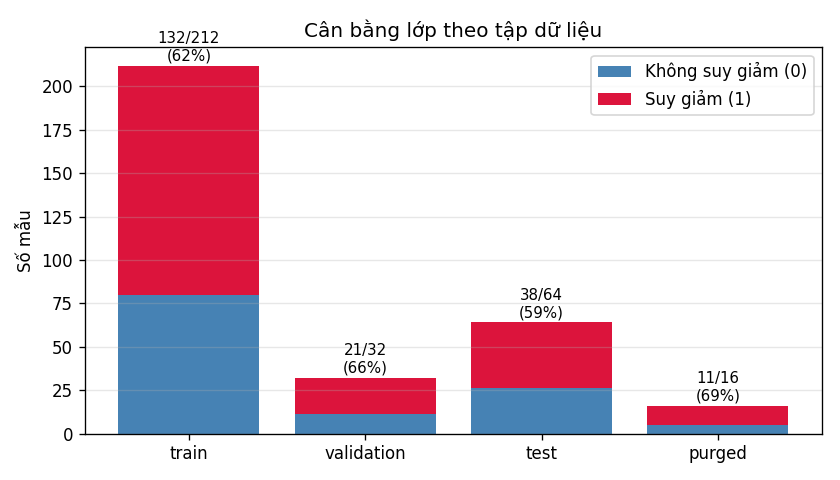
\includegraphics[width=0.78\textwidth]{figures/class_balance.png}
\caption{Cân bằng lớp theo tập dữ liệu}
\label{fig:class_balance}
\end{figure}

\begin{figure}[H]
\centering
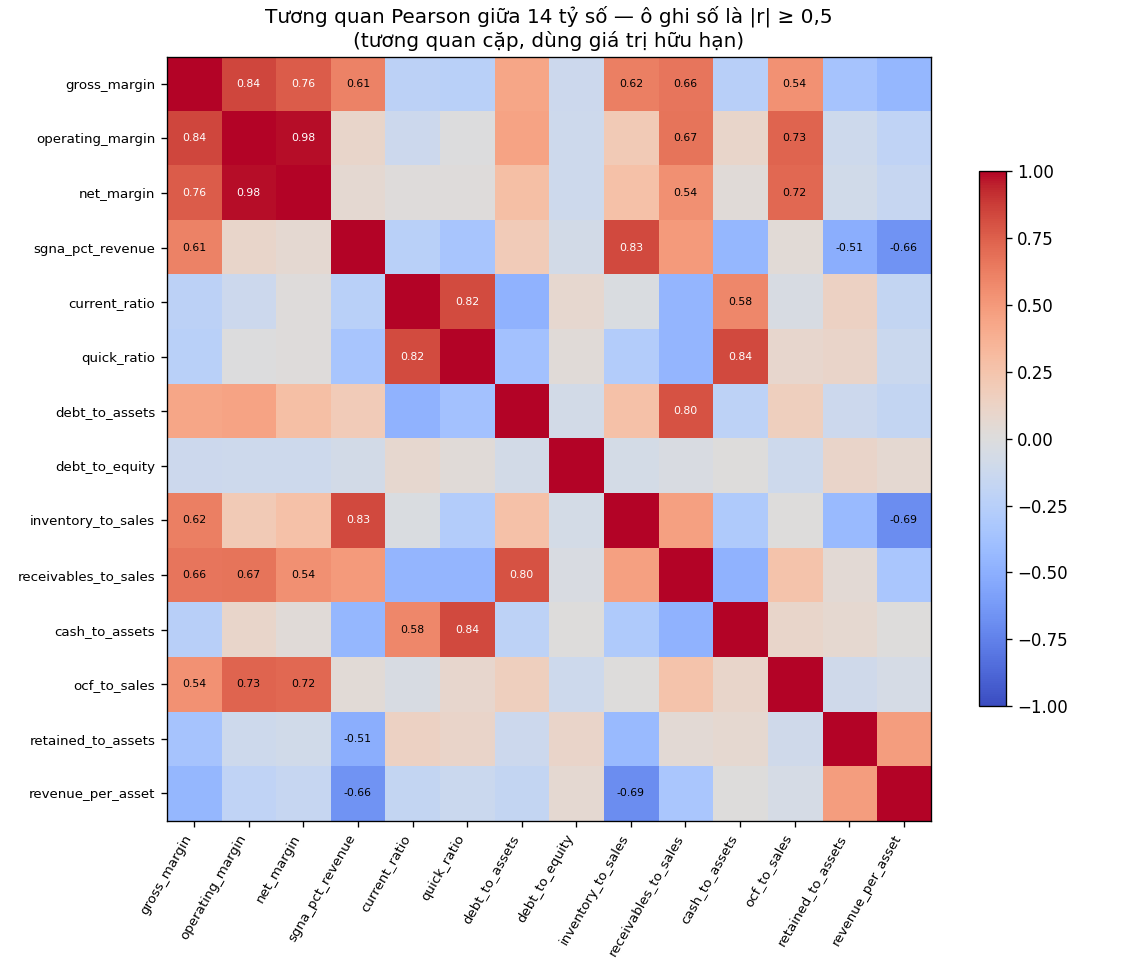
\includegraphics[width=0.78\textwidth]{figures/ratio_correlation.png}
\caption{Tương quan giữa các tỷ số tài chính}
\label{fig:ratio_corr}
\end{figure}

\subsection{Mười bốn tỷ số tài chính}

Các tỷ số (từ điển \texttt{RATIOS} trong \texttt{forecasting/config.py}) chia bốn nhóm kinh tế:

\begin{itemize}
\item \textbf{Thanh khoản:} \texttt{current\_ratio} $=$ tài sản ngắn hạn / nợ ngắn hạn;
      \texttt{quick\_ratio} $=$ (tài sản ngắn hạn $-$ hàng tồn kho) / nợ ngắn hạn.
\item \textbf{Đòn bẩy:} \texttt{debt\_to\_assets} $=$ nợ / tổng tài sản; \texttt{debt\_to\_equity}
      $=$ nợ / vốn chủ sở hữu.
\item \textbf{Sinh lời:} \texttt{gross\_margin} $=$ (doanh thu $-$ giá vốn) / doanh thu;
      \texttt{operating\_margin} $=$ lợi nhuận hoạt động / doanh thu; \texttt{net\_margin} $=$ lợi
      nhuận ròng / doanh thu; \texttt{retained\_to\_assets} $=$ lợi nhuận giữ lại / tổng tài sản.
\item \textbf{Hiệu quả hoạt động:} \texttt{inventory\_to\_sales}, \texttt{receivables\_to\_sales},
      \texttt{revenue\_per\_asset}, \texttt{ocf\_to\_sales}, \texttt{sgna\_pct\_revenue},
      \texttt{cash\_to\_assets}.
\end{itemize}

Mỗi tỷ số được đưa vào mô hình ở hai dạng: giá trị của quý gần nhất (\texttt{*\_latest}) và mức thay
đổi so với cùng kỳ năm trước (\texttt{*\_yoy}), tức $14 \times 2 = 28$ cột.

\subsection{Tăng trưởng, cấu trúc vốn và đặc trưng đường đi}

Nhóm tăng trưởng gồm 10 cột \texttt{*\_yoy\_growth} cho các chỉ tiêu chính. Nhóm cấu trúc vốn có
\texttt{working\_capital\_to\_assets}. Nhóm đường đi (\texttt{path}) là phần thiết kế riêng cho bài
toán này: vì suy giảm tài chính là một quá trình, khóa luận đưa vào cực trị xấu nhất trong cửa sổ và
số quý âm liên tiếp — \texttt{current\_ratio\_min\_window}, \texttt{ocf\_to\_sales\_min\_window},
\texttt{net\_margin\_min\_window}, \texttt{revenue\_drawdown\_window},
\texttt{negative\_ni\_streak}, \texttt{negative\_ocf\_streak}.

\begin{table}[H]
\centering
\caption{Cấu trúc 47 đặc trưng theo nhóm}
\label{tab:feature_groups}
\begin{tabular}{|l|r|l|}
\hline
\textbf{Nhóm} & \textbf{Số cột} & \textbf{Nội dung} \\
\hline
ratios\_latest & 14 & 14 tỷ số tại quý gần nhất \\
ratios\_yoy    & 14 & Mức thay đổi so với cùng kỳ \\
growth         & 10 & Tăng trưởng YoY của 10 chỉ tiêu chính \\
structure      & 1  & working\_capital\_to\_assets \\
stress         & 2  & distress\_quarters\_in\_window, revenue\_cv \\
path           & 6  & Cực trị xấu nhất + số quý âm liên tiếp \\
\hline
\textbf{Tổng}  & \textbf{47} & \\
\hline
\end{tabular}
\end{table}

\subsection{Xử lý giá trị khuyết và ngoại lai}

Giá trị khuyết giữ nguyên dạng NaN qua tầng đặc trưng, rồi xử lý bên trong pipeline bằng
\texttt{SimpleImputer(strategy='median')}, với median tính chỉ trên train. Với ngoại lai, khóa luận
thử \texttt{Winsorizer} (clip theo IQR hoặc P1--P99, ngưỡng học từ train) như một biến thể và báo
cáo kết quả âm: trên đúng mô hình được chốt (Random Forest), winsorize IQR cải thiện AP
cross-company chỉ $+0{,}13$ điểm \% (0,9590 so với 0,9577) — nằm trong khoảng nhiễu của 244 mẫu
out-of-fold. Vì vậy pipeline chính giữ không winsorize cho đơn giản và dễ diễn giải; winsorize chỉ
dùng như một ablation. Kết quả tương tự với lựa chọn scaler: \texttt{StandardScaler} và
\texttt{RobustScaler} chênh nhau dưới 0,5 điểm \% AP cross-company.

\section{Thiết kế mô hình học máy}
\label{sec:models}

\subsection{Bốn họ mô hình}

Khóa luận cố tình chọn bốn họ mô hình khác nhau về cơ chế học để trả lời câu hỏi "bài toán cần loại
giả thuyết nào", thay vì thử nhiều biến thể của cùng một họ: tuyến tính (Logistic Regression),
bagging cây (Random Forest), boosting cây (HistGradientBoosting) và mạng nơ-ron phi tuyến không dựa
trên cây (MLP). Toàn bộ dùng thư viện \texttt{scikit-learn}; pipeline chính không dùng
\texttt{xgboost}/\texttt{lightgbm}.

\begin{table}[H]
\centering
\caption{Siêu tham số của bốn họ mô hình}
\label{tab:hyperparams}
\begin{tabular}{|l|l|p{7.4cm}|}
\hline
\textbf{Mô hình} & \textbf{Lớp scikit-learn} & \textbf{Siêu tham số mặc định} \\
\hline
Logistic Regression & LogisticRegression & max\_iter=2000, C=0,1 \\
Random Forest & RandomForestClassifier & n\_estimators=300, max\_depth=6,
min\_samples\_leaf=2, class\_weight=balanced\_subsample \\
HistGradientBoosting & HistGradientBoostingClassifier & max\_iter=300, learning\_rate=0,05,
max\_depth=3, l2\_regularization=1,0, class\_weight=balanced \\
MLP & MLPClassifier & hidden\_layer\_sizes=32, alpha=1e-3, learning\_rate\_init=1e-3,
early\_stopping=True \\
\hline
\end{tabular}
\end{table}

Lưu ý kỹ thuật với mất cân bằng: \texttt{RandomForestClassifier} và
\texttt{HistGradientBoostingClassifier} nhận \texttt{class\_weight} nên trọng số lớp được truyền
trực tiếp. \texttt{MLPClassifier} không có \texttt{class\_weight}, nên mất cân bằng được xử lý bằng
ngưỡng/cost-sensitive ở tầng đánh giá thay vì nhồi trọng số giả vào mô hình.

\subsection{Pipeline và kiểm soát rò rỉ dữ liệu}

Mỗi mô hình là một \texttt{sklearn.pipeline.Pipeline}:
\texttt{[winsorize] $\rightarrow$ SimpleImputer(median) $\rightarrow$ [scaler] $\rightarrow$ model}
(hàm \texttt{make\_model} trong \texttt{forecasting/models.py}). Đặt bước impute và scale bên trong
Pipeline có tác dụng chặn rò rỉ: thống kê impute/scale chỉ được \texttt{fit} trên train, và khi kiểm
định chéo chỉ trên fold-train. Scaler mặc định là \texttt{StandardScaler} cho mô hình tuyến
tính/MLP và \texttt{none} cho mô hình cây. \texttt{RANDOM\_SEED = 42} được cố định để tái lập.

\subsection{Quy tắc chọn mô hình}

Nếu chọn mô hình theo AUROC in-domain, kết quả sẽ bị chi phối bởi việc "nhớ mặt công ty" — baseline
ticker-prior đạt AUROC 0,986 (mục~\ref{sec:baseline}). Vì vậy quy tắc chọn theo thứ tự ưu tiên:
\textbf{AP cross-company} (GroupKFold trên train+validation) $\rightarrow$ best-F1(validation)
$\rightarrow$ AP(validation) $\rightarrow$ AUROC(validation) $\rightarrow$ gap overfit nhỏ nhất. Quy
tắc này được mã hoá tại \texttt{forecasting/train.py::\_rank} và ghi lại trong \texttt{summary.json}
để kiểm chứng được.

\subsection{Tinh chỉnh siêu tham số}

Tinh chỉnh dùng kiểm định chéo chia theo công ty (\texttt{GroupKFold}) và chọn theo AP, để không lặp
lại sai lầm chọn theo metric in-domain. Nhận xét trung thực: kết quả tinh chỉnh chênh lệch rất nhỏ
so với cấu hình mặc định — mô hình RF tốt nhất (\texttt{max\_depth=3, n\_estimators=500}) chỉ hơn
mặc định $+0{,}3$ điểm \% CV-AP; MLP hơn $+4{,}6$ điểm \% nhưng vẫn tụt hậu về cross-company. Vì
vậy mô hình triển khai giữ cấu hình mặc định (đơn giản, ít nguy cơ overfit do lựa chọn), và bảng
tinh chỉnh được giữ lại như bằng chứng là nhóm đã thử.

\begin{table}[H]
\centering
\caption{Tinh chỉnh siêu tham số, kiểm định chéo chia theo công ty}
\label{tab:tuning}
\begin{tabular}{|l|l|r|r|}
\hline
\textbf{Mô hình} & \textbf{Cấu hình tốt nhất} & \textbf{CV-AP} & \textbf{CV-AUROC} \\
\hline
logistic & C=0,01, class\_weight=None & 0,960 & 0,917 \\
random\_forest & max\_depth=3, min\_samples\_leaf=2, n\_estimators=500 & 0,989 & 0,976 \\
hist\_gradient\_boosting & learning\_rate=0,03, max\_depth=2, max\_iter=200 & 0,939 & 0,934 \\
mlp & alpha=1e-4, hidden\_layer\_sizes=64 & 0,845 & 0,750 \\
\hline
\end{tabular}
\end{table}



% =====================================================================
%  CHƯƠNG 4 — TRÌNH BÀY VÀ ĐÁNH GIÁ BÀN LUẬN KẾT QUẢ
% =====================================================================
\chapter{Trình bày và đánh giá bàn luận kết quả}

Mọi so sánh trong chương dùng cùng tập test 64 mẫu (38 dương, 59,4\%), và test không tham gia vào
bất kỳ bước chọn mô hình hay chọn ngưỡng nào.

\section{Kết quả thực nghiệm}

\subsection{So sánh bốn họ mô hình}

\begin{table}[H]
\centering
\caption{Bốn họ mô hình trên test tại ngưỡng vận hành 0,788}
\label{tab:four_models}
\begin{tabular}{|l|r|r|r|r|r|l|}
\hline
\textbf{Mô hình} & \textbf{AUROC} & \textbf{AP} & \textbf{F1@0,5} & \textbf{F1@0,788} &
\textbf{MCC@0,788} & \textbf{TN/FP/FN/TP} \\
\hline
Logistic Regression  & 0,983 & 0,989 & 0,935 & 0,914 & 0,827 & 26/0/6/32 \\
Random Forest        & 0,983 & 0,991 & 0,949 & 0,960 & 0,904 & 25/1/2/36 \\
HistGradientBoosting & 0,977 & 0,987 & 0,937 & 0,907 & 0,775 & 23/3/4/34 \\
MLP                  & 0,971 & 0,982 & 0,914 & 0,895 & 0,741 & 22/4/4/34 \\
\hline
\end{tabular}
\end{table}

Random Forest là mô hình được chốt. Tại ngưỡng 0,788, nó đạt precision $= 0{,}973$,
recall $= 0{,}947$, F1 $= 0{,}960$, accuracy $= 0{,}953$, specificity $= 0{,}962$ và Brier
$= 0{,}058$. Đáng chú ý là cả bốn họ mô hình đều cho F1@0,5 khá cao (0,91--0,95) nhưng chỉ 1--2 mô
hình giữ được F1 cao khi ngưỡng dịch lên 0,788 — nghĩa là thứ hạng điểm số giữa các mô hình không
khác nhiều, khác biệt nằm ở vùng xác suất quanh ngưỡng quyết định.

\begin{figure}[H]
\centering
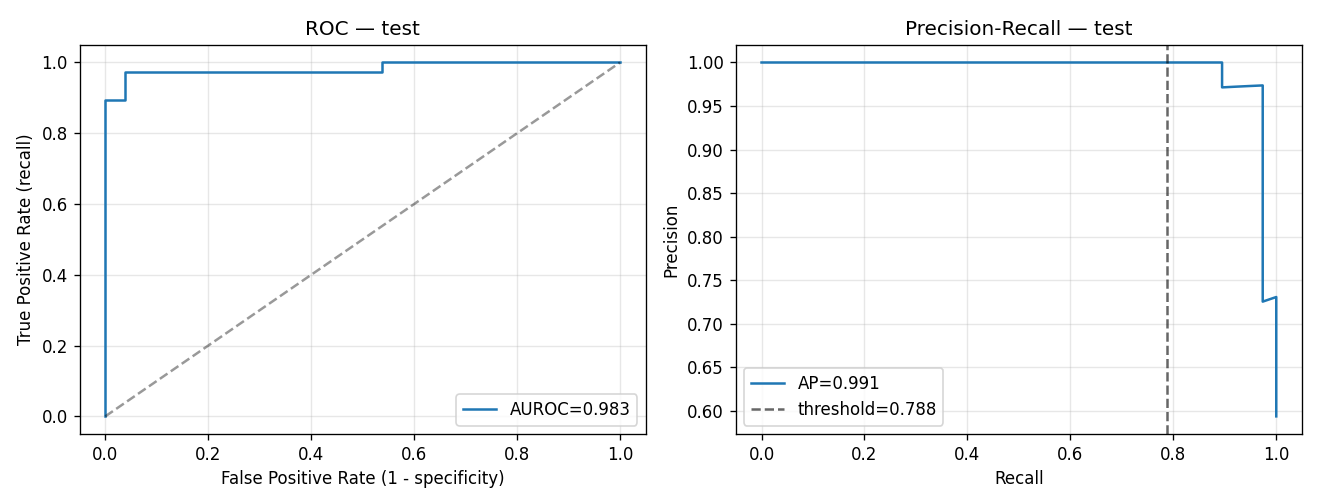
\includegraphics[width=0.72\textwidth]{figures/roc_pr_curves.png}
\caption{Đường ROC và Precision--Recall trên tập test}
\label{fig:roc_pr}
\end{figure}

\subsection{So sánh với baseline và giao thức chống thổi phồng}
\label{sec:baseline}

Đây là phần quan trọng nhất về mặt phương pháp. Nếu chỉ nhìn AUROC $\approx 0{,}98$, ta dễ kết luận
mô hình rất tốt. Nhưng đặt cạnh một baseline không dùng mô hình — lấy tỉ lệ nhãn 1 trung bình trong
train theo từng công ty (\texttt{ticker\_prior}) — mô hình gần như không hơn.

\begin{table}[H]
\centering
\caption{So sánh mô hình chốt với các hệ thống đối chứng}
\label{tab:baselines}
\begin{tabular}{|l|r|r|}
\hline
\textbf{Hệ thống} & \textbf{AUROC} & \textbf{AP} \\
\hline
model[random\_forest]                  & 0,983 & 0,991 \\
ticker\_prior (baseline không học)     & 0,986 & 0,985 \\
single\_feature[debt\_to\_assets]      & 0,889 & 0,938 \\
rule[Altman $Z'' < 1{,}1$]             & 0,758 & 0,865 \\
dummy\_most\_frequent                  & 0,500 & 0,594 \\
\hline
\end{tabular}
\end{table}

Baseline ticker-prior ngang bằng hoặc nhích hơn mô hình về AUROC (0,986 so với 0,983) và chỉ kém
hơn về AP (0,985 so với 0,991). Quy tắc Altman $Z''$ đạt AUROC 0,758 — thấp hơn rõ rệt nhưng dùng
công thức công khai, không học tham số và không cần huấn luyện. Để tách phần "nhớ mặt công ty" khỏi
năng lực tổng quát hoá, khóa luận đánh giá lại theo \texttt{GroupKFold} (giữ trọn một công ty ra
ngoài train trong mỗi fold).

\begin{table}[H]
\centering
\caption{In-domain so với cross-company (GroupKFold)}
\label{tab:cross_company}
\begin{tabular}{|l|r|r|r|r|}
\hline
\textbf{Mô hình} & \textbf{AUROC in-domain} & \textbf{AP in-domain} &
\textbf{AUROC cross-co.} & \textbf{AP cross-co.} \\
\hline
Random Forest        & 0,983 & 0,991 & 0,933 & 0,957 \\
Logistic Regression  & 0,983 & 0,989 & 0,912 & 0,942 \\
HistGradientBoosting & 0,977 & 0,987 & 0,926 & 0,953 \\
MLP                  & 0,971 & 0,982 & 0,789 & 0,832 \\
\hline
\end{tabular}
\end{table}

Hai điểm cần nói thẳng. Thứ nhất, khi giữ công ty ra ngoài, AUROC của mô hình chốt giảm từ 0,983
xuống 0,933 — mức sụt này cho biết một phần đáng kể hiệu năng in-domain đến từ việc nhận diện công
ty. Thứ hai, MLP sụt mạnh nhất (0,971 $\rightarrow$ 0,789): mạng nơ-ron tận dụng tốt các đặc trưng
gần như bất biến theo công ty nên khi công ty bị giữ trọn ra ngoài thì mất chỗ dựa. Thêm một phép
thử khắt khe là \texttt{Leave-One-Company-Out}: AUROC trung bình chỉ 0,628.

\subsection{Ngưỡng quyết định theo chi phí kỳ vọng}

\begin{table}[H]
\centering
\caption{Ngưỡng theo F1 và theo chi phí kỳ vọng}
\label{tab:threshold}
\begin{tabular}{|l|r|r|r|r|r|}
\hline
\textbf{Tập} & \textbf{Ngưỡng best-F1} & \textbf{F1} & \textbf{Precision} & \textbf{Recall} &
\textbf{Chi phí kỳ vọng} \\
\hline
validation & 0,788 & 0,976 & 1,000 & 0,952 & 5,0 \\
test       & 0,783 & 0,974 & 0,974 & 0,974 & 6,0 \\
\hline
\end{tabular}
\end{table}

Điểm cần nói thẳng: ngưỡng triển khai 0,788 lấy từ validation, trong khi trên test ngưỡng tối ưu chi
phí là 0,783. Chỉ lệch 0,005 nhưng trên 64 mẫu nó biến 1 dương tính thật thành bỏ sót: tại 0,788,
ma trận nhầm lẫn là TN/FP/FN/TP $= 25/1/2/36$; tại 0,783 là $25/1/1/37$. Đây là biểu hiện rõ của việc
chọn ngưỡng trên một tập nhỏ rồi áp lên tập khác — không sai về giao thức, nhưng cần đọc kèm khoảng
tin cậy thay vì tin vào một con số duy nhất.

\subsection{Kiểm định ý nghĩa thống kê và độ nhạy theo định nghĩa nhãn}

Để tránh kết luận "mô hình tốt hơn" chỉ dựa vào chênh lệch điểm số, khóa luận kiểm định trên cùng 64
mẫu test: DeLong \cite{delong1988} cho $\Delta$AUROC và paired bootstrap (2.000 vòng) cho
$\Delta$AP.

\begin{table}[H]
\centering
\caption{Kiểm định mô hình chốt so với các hệ thống khác}
\label{tab:significance}
\begin{tabular}{|l|r|r|r|l|r|}
\hline
\textbf{So sánh (A $-$ B)} & \textbf{$\Delta$AUROC} & \textbf{p (DeLong)} & \textbf{$\Delta$AP} &
\textbf{CI95 $\Delta$AP} & \textbf{p (bootstrap)} \\
\hline
RF $-$ ticker\_prior        & $-0{,}0030$ & 0,755  & $+0{,}0061$ & $[-0{,}005; +0{,}022]$ & 0,344 \\
RF $-$ single\_feature      & $+0{,}0941$ & 0,0076 & $+0{,}0528$ & $[+0{,}018; +0{,}097]$  & 0,001 \\
RF $-$ dummy\_most\_frequent& $+0{,}4828$ & $<0{,}001$ & $+0{,}3970$ & $[+0{,}379; +0{,}406]$ & $<0{,}001$ \\
\hline
\end{tabular}
\end{table}

Kết quả then chốt: mô hình chốt không khác baseline ticker-prior về ý nghĩa thống kê (p $=$ 0,755 cho
AUROC; p $=$ 0,344 cho AP, khoảng tin cậy chứa 0). Cần đọc đúng: "không khác biệt" nghĩa là dữ liệu
chưa đủ để khẳng định mô hình hơn, không phải bằng chứng mô hình kém. Với $n = 64$, khoảng tin cậy
vốn rộng.

\subsection{Kiểm chứng độ nhạy theo định nghĩa nhãn}
\label{sec:nhan}

Nhóm dựng lại toàn bộ split bằng ba định nghĩa nhãn công khai, tái lập được (\texttt{stress\_signals},
Altman $Z''$, forward 4 quý) và chạy lại đúng một mô hình.

\begin{table}[H]
\centering
\caption{Kiểm chứng độ nhạy theo định nghĩa nhãn}
\label{tab:label_sensitivity}
\begin{tabular}{|l|r|r|r|r|r|}
\hline
\textbf{Định nghĩa nhãn} & \textbf{Dương (test)} & \textbf{Khớp nhãn gốc} &
\textbf{AUROC mô hình} & \textbf{AUROC ticker-prior} & \textbf{Cross-co. AP} \\
\hline
original (nhãn gốc) & 59,4\% & 100\% & 0,983 & 0,986 & 0,958 \\
stress\_signals     & 42,2\% & 74,4\%& 0,909 & 0,960 & 0,610 \\
altman\_z           & 31,2\% & 63,9\%& 0,999 & 0,991 & 0,460 \\
forward\_4q         & 48,4\% & 66,7\%& 0,836 & 0,911 & 0,582 \\
\hline
\end{tabular}
\end{table}

Luận điểm "mô hình không vượt baseline nhớ mặt công ty" xuất hiện ở 3/3 định nghĩa nhãn tái lập được
— đây là bằng chứng mạnh nhất của khóa luận: kết luận không phụ thuộc vào cách gán nhãn. Đồng thời,
cross-company AP sụt rất mạnh ở các định nghĩa khác (0,46--0,61), xác nhận lại rằng phần lớn hiệu
năng in-domain đến từ thực thể chứ không từ động lực suy giảm của từng quý.

\subsection{Thực nghiệm phản biện}

Để trả lời câu hỏi "có phải do chọn họ mô hình nên chưa hơn baseline?", khóa luận chạy thêm hai đối
chứng ngoài pipeline chính: một SVM tuyến tính nhẹ (LiteSVM, cài bằng numpy) và XGBoost
\cite{chen2016}.

\begin{table}[H]
\centering
\caption{Mô hình chốt so với LiteSVM và XGBoost}
\label{tab:defense}
\begin{tabular}{|l|r|r|l|}
\hline
\textbf{Mô hình} & \textbf{Test AUROC} & \textbf{Test AP} & \textbf{TN/FP/FN/TP} \\
\hline
LiteSVM (SGD hinge + class\_weight) & 0,965 & 0,976 & 26/0/19/19 \\
XGBoost (scale\_pos\_weight + early stop) & 0,982 & 0,990 & 26/0/4/34 \\
Random Forest (khóa luận) & 0,983 & 0,991 & 25/1/2/36 \\
\hline
\end{tabular}
\end{table}

XGBoost đạt AUROC/AP tương đương Random Forest trong khi không có FP nào (bỏ sót 4) — việc thay
boosting bằng bagging không tạo khác biệt lớn trên bộ dữ liệu này. Khóa luận cũng chạy thí nghiệm xử
lý mất cân bằng trên dữ liệu thật (SMOTE \cite{chawla2002}, SMOTE+ENN, RandomUnderSampler,
class\_weight) đặt trong \texttt{imblearn.pipeline.Pipeline} \cite{lemaitre2017} để không chạm test;
kỹ thuật tốt nhất (\texttt{smote\_enn}, AP 0,9683 so với 0,9588 của đối chứng) nhưng $\Delta$AP
$= +0{,}0095$ với p $= 0{,}21$ — chưa đủ căn cứ. Một chi tiết đáng lưu ý: vì lớp 1 chiếm đa số
(62\%), SMOTE ở đây sinh thêm mẫu lớp 0, tức can thiệp ngược với thực hành phổ biến — thêm một lý do
để mất cân bằng không phải nút thắt của bài toán này.

\section{Phân tích độ quan trọng đặc trưng và SHAP}

\subsection{Permutation importance}

Khóa luận dùng permutation importance \cite{fisher2019} (hoán vị từng cột, đo mức giảm AUROC). Kết
quả trên validation ở Bảng~\ref{tab:importance}.

\begin{table}[H]
\centering
\caption{Độ quan trọng đặc trưng (permutation, $\Delta$AUROC trên validation)}
\label{tab:importance}
\begin{tabular}{|r|l|r|}
\hline
\textbf{Hạng} & \textbf{Đặc trưng} & \textbf{$\Delta$AUROC (val)} \\
\hline
1 & gross\_margin\_latest            & 0,008 \\
2 & receivables\_to\_sales\_latest   & 0,001 \\
3 & working\_capital\_to\_assets     & 0,001 \\
4 & operating\_margin\_latest        & 0,001 \\
5 & net\_margin\_latest              & 0,000 \\
6 & retained\_to\_assets\_latest     & 0,000 \\
\hline
\end{tabular}
\end{table}

Các $\Delta$AUROC đều rất nhỏ ($\leq 0{,}008$) — nghĩa là khi công ty đã được nhận diện, không đặc
trưng đơn lẻ nào còn đóng góp lớn. Đặc trưng dẫn đầu là \texttt{gross\_margin\_latest} (biên lợi
nhuận gộp), hợp lý với ngành bán lẻ vì đây là tỷ số phản ứng nhanh nhất với áp lực giá và cơ cấu
hàng tồn.

\begin{figure}[H]
\centering
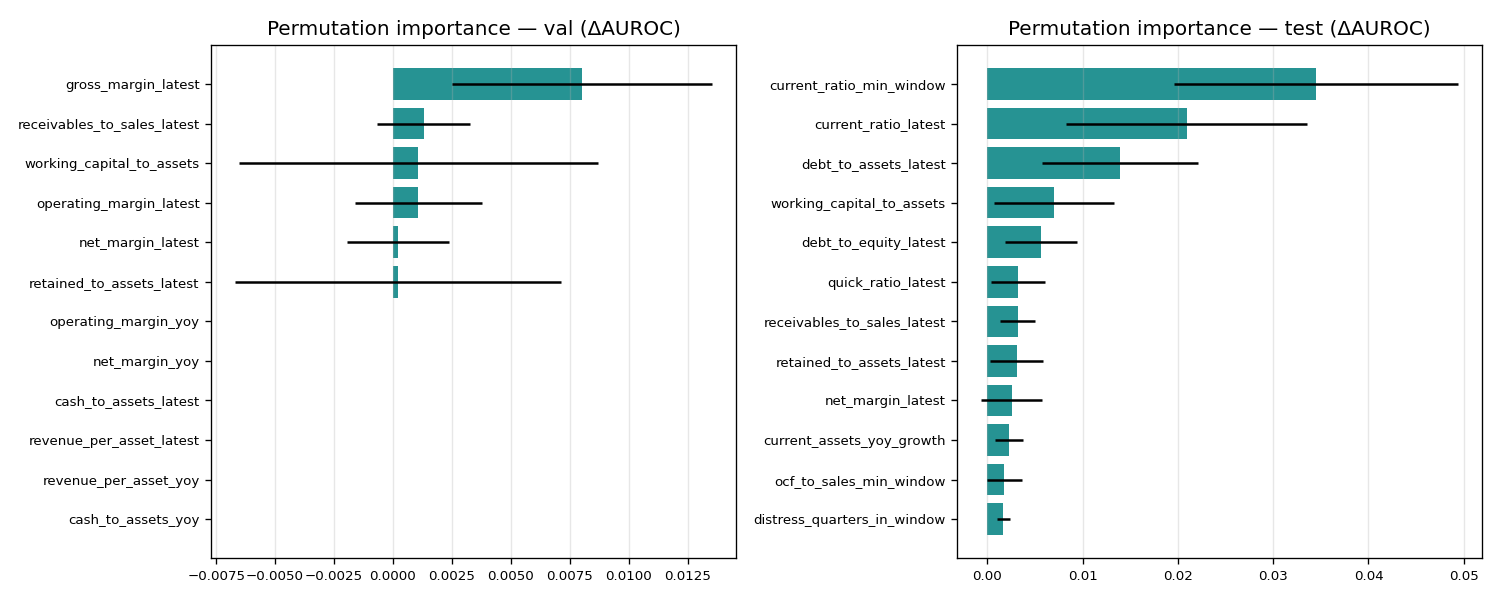
\includegraphics[width=0.74\textwidth]{figures/feature_importance.png}
\caption{Độ quan trọng đặc trưng (permutation importance)}
\label{fig:importance}
\end{figure}

\subsection{Ablation theo nhóm đặc trưng}

\begin{table}[H]
\centering
\caption{Ablation theo nhóm đặc trưng (test)}
\label{tab:ablation}
\begin{tabular}{|l|r|r|r|r|}
\hline
\textbf{Biến thể} & \textbf{Số đặc trưng} & \textbf{AUROC} & \textbf{AP} & \textbf{F1} \\
\hline
Tất cả đặc trưng        & 47 & 0,983 & 0,991 & 0,949 \\
Bỏ nhóm ratios\_latest  & 33 & 0,966 & 0,982 & 0,949 \\
Bỏ nhóm ratios\_yoy     & 33 & 0,974 & 0,985 & 0,949 \\
Bỏ nhóm growth          & 37 & 0,985 & 0,993 & 0,949 \\
Bỏ nhóm path            & 41 & 0,977 & 0,987 & 0,949 \\
Chỉ mẫu $\geq 5$ quý     & 47 & 0,987 & 0,993 & 0,949 \\
\hline
\end{tabular}
\end{table}

Ablation cho thấy F1 test gần như không đổi (0,949) ở mọi biến thể, còn AUROC dao động trong khoảng
$\pm 0{,}02$ — kết luận không nhạy với việc bỏ nguyên một nhóm đặc trưng. Bỏ nhóm
\texttt{ratios\_latest} làm AUROC giảm nhiều nhất (0,983 $\rightarrow$ 0,966), cho thấy giá trị tỷ số
tại quý gần nhất là phần thông tin cốt lõi. Một cảnh báo kỹ thuật đi kèm: đa cộng tuyến cao —
33/47 đặc trưng có VIF $>$ 10, nặng nhất là \texttt{debt\_to\_equity} và các cột \texttt{cash\_*}.
Với mô hình tuyến tính, VIF cao làm hệ số bất ổn và khó diễn giải; với mô hình cây thì ít ảnh hưởng
đến dự báo nhưng vẫn làm độ quan trọng bị chia đều giữa các cột tương quan.

\subsection{Giải thích cục bộ bằng SHAP}

Ngoài độ quan trọng toàn cục, khóa luận dùng KernelSHAP tự cài đặt \cite{lundberg2017} để giải thích
từng ca dự báo: với mỗi mẫu, tính đóng góp của từng đặc trưng vào độ lệch so với giá trị nền. Phần
này được dùng chủ yếu cho ứng dụng minh hoạ và kiểm tra tính hợp lý, không dùng để chọn mô hình —
lý do là SHAP tính trên mô hình đã fit, nếu dùng để chọn cây sẽ quay lại đúng vấn đề thổi phồng
in-domain đã nêu ở mục~\ref{sec:baseline}.

\begin{figure}[H]
\centering
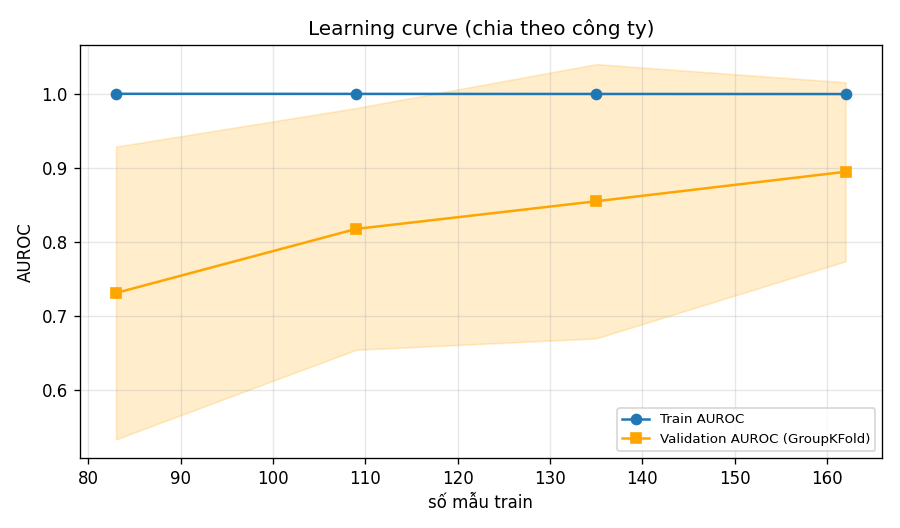
\includegraphics[width=0.76\textwidth]{figures/learning_curve.png}
\caption{Learning curve khi chia theo công ty}
\label{fig:learning_curve}
\end{figure}

\section{Phân tích lỗi và thảo luận}

\subsection{Phân tích lỗi (error analysis)}

Trên test, mô hình chốt sai 3/64 mẫu. Bảng~\ref{tab:errors} truy vết từng ca tới chỉ tiêu cụ thể.

\begin{table}[H]
\centering
\caption{Ba mẫu dự đoán sai trên tập test}
\label{tab:errors}
\begin{tabular}{|l|l|r|l|r|r|r|r|}
\hline
\textbf{Mẫu} & \textbf{Cty} & \textbf{Thực} & \textbf{Dự đoán} & \textbf{P} &
\textbf{current\_r.} & \textbf{WC/TA} & \textbf{net\_m.} \\
\hline
HD-2024Q2   & HD   & 1 & 0 (FN) & 0,783 & 1,34 & 0,10 & 0,099 \\
DG-2025Q2   & DG   & 0 & 1 (FP) & 0,798 & 1,23 & 0,05 & 0,038 \\
FIVE-2024Q3 & FIVE & 1 & 0 (FN) & 0,174 & 1,63 & 0,11 & 0,040 \\
\hline
\end{tabular}
\end{table}

Ba ca này lộ ra đúng bản chất vấn đề. HD-2024Q2 là bỏ sót sát ngưỡng: HD có 100\% quý mang nhãn 1,
nhưng quý này các tỷ số lại khá hơn (net\_margin 0,099; debt/assets 0,98) nên xác suất 0,783 nằm
ngay dưới ngưỡng 0,788 — mô hình gần như dựa vào danh tính công ty chứ không vào tín hiệu của quý.
FIVE-2024Q3 là bỏ sót nặng (0,174): đây là lỗi đáng lo nhất, vì mô hình không hề thấy dấu hiệu nào.
DG-2025Q2 là báo động giả (0,798) ở một công ty có nhãn lẫn lộn. Điểm chung: cả ba mẫu đều thuộc các
công ty có tỉ lệ nhãn trung gian, nơi ranh giới quyết định mờ.

\begin{figure}[H]
\centering
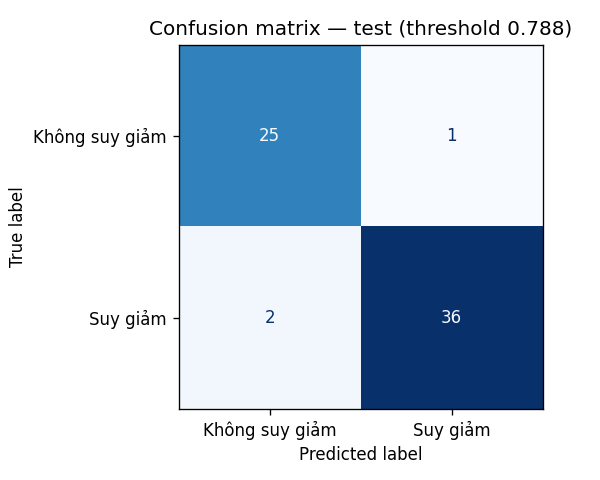
\includegraphics[width=0.52\textwidth]{figures/confusion_matrix.png}
\caption{Ma trận nhầm lẫn của mô hình chốt trên tập test}
\label{fig:confusion}
\end{figure}

\subsection{Rào cản kỹ thuật khi triển khai thực tế}

\begin{enumerate}
\item \textbf{Độ trễ dữ liệu theo quý.} Đầu vào là báo cáo quý đã công bố. 10-Q thường được nộp
      sau khi quý kết thúc khoảng 40 ngày, 10-K có kiểm toán; mọi đặc trưng dùng mốc
      \texttt{available\_on} $=$ ngày \texttt{filed}. Điều đó có nghĩa dự báo chỉ có thể đưa ra SAU
      khi báo cáo được nộp, mô hình không thể cảnh báo sớm hơn chính dữ liệu. Tệ hơn, các tỷ số kế
      toán là chỉ báo trễ: khi chúng xấu đi thì vấn đề thường đã xảy ra rồi.
\item \textbf{Rò rỉ thông tin cấp thực thể.} Đây là rủi ro lớn nhất về phương pháp. Nếu chia tập
      ngẫu nhiên theo mẫu, cùng một công ty xuất hiện ở cả train lẫn test và mô hình chỉ cần nhớ
      mặt công ty là đủ đạt điểm cao giả tạo. Khóa luận tránh bằng chia theo thời gian, GroupKFold,
      LOCO và luôn so với baseline ticker-prior.
\item \textbf{Chi phí sai không đối xứng.} Trong ứng dụng đầu tư/cho vay, một false negative (bỏ
      sót doanh nghiệp sắp suy giảm) đắt hơn một false positive. Khóa luận xử lý bằng ngưỡng tối ưu
      chi phí, nhưng giả định $C_{FN} = 5$ là con số minh hoạ, không phải con số đo từ thị trường.
\item \textbf{Nhãn mục tiêu không tái tạo được.} Không quy tắc kế toán đơn giản nào khớp nhãn gốc
      quá 74,7\%. Điều này giới hạn khả năng kiểm chứng độc lập và buộc khóa luận phải kiểm chứng
      độ nhạy bằng các định nghĩa nhãn thay thế.
\item \textbf{Nguy cơ overfitting.} Random Forest đạt AUROC train 1,000 nhưng validation 0,965
      (gap 0,034); learning curve chia theo công ty cho gap khoảng 0,105 AUROC. Với 212 mẫu train và
      47 đặc trưng, đây là mức overfit cần theo dõi, và là lý do khóa luận không dùng cấu hình tinh
      chỉnh phức tạp.
\end{enumerate}

\subsection{Ý nghĩa thực tiễn và hạn chế}

Giá trị thực dụng rõ nhất không nằm ở con số AUROC 0,983, mà ở hai thứ khác. Thứ nhất là khả năng tự
động hoá bóc tách: thay vì đọc 8 $\times$ 44 báo cáo, pipeline lấy thẳng \texttt{companyfacts},
chuẩn hoá kỳ kế toán, tính 47 đặc trưng và gán nhãn, tất cả tái lập được từ một lệnh. Thứ hai là
phát hiện trung thực về rò rỉ cấp thực thể: bất kỳ ai triển khai dự báo suy giảm trên bộ dữ liệu ít
thực thể đều cần biết rằng AUROC in-domain có thể cao phần lớn do nhận diện công ty.

Về hạn chế: cỡ mẫu nhỏ và chỉ 8 thực thể nên mọi kết luận phải đi kèm khoảng tin cậy và không suy
rộng ra toàn ngành; chuỗi thời gian bị chồng lấn giữa các mẫu liên tiếp nên số quan sát độc lập thực
tế nhỏ hơn 324; nhãn gốc không tái tạo được; đơn vị tiền chỉ là quy đổi minh hoạ; và bộ dữ liệu
không chứa sự kiện phá sản thật, nên kết quả không thể diễn giải thành năng lực dự báo phá sản.




% =====================================================================
%  CHƯƠNG 5 — KẾT LUẬN VÀ HƯỚNG PHÁT TRIỂN
% =====================================================================
\chapter{Kết luận và hướng phát triển}

\section{Kết luận}

Khóa luận đã làm được những việc cụ thể và chưa chứng minh được một điều quan trọng. Về phần đã làm:

\begin{itemize}
\item Pipeline dữ liệu SEC XBRL tái lập được: 8 công ty, 332 quý, 16 chỉ tiêu, kiểm chứng nguồn gốc
      bằng SHA-256 (0 hash lệch, 0 fact thiếu, 0 ô bịa số).
\item Bộ 47 đặc trưng tài chính gồm tỷ số thanh khoản/đòn bẩy/sinh lời/hiệu quả, tăng trưởng so với
      cùng kỳ và đặc trưng đường đi theo cửa sổ quý.
\item Bốn họ mô hình scikit-learn đặt trong một Pipeline chống rò rỉ, cộng các baseline đối chứng
      (dummy, ticker-prior, single-feature, Altman $Z''$).
\item Kết quả trên test: Random Forest được chốt đạt AUROC 0,983, AP 0,991, F1 0,960 tại ngưỡng vận
      hành 0,788.
\item Ba lớp kiểm chứng: cross-company/LOCO, kiểm định ý nghĩa (DeLong và bootstrap), và kiểm chứng
      độ nhạy theo ba định nghĩa nhãn tái lập được.
\end{itemize}

Về phần chưa chứng minh được — và đây là kết luận trung thực quan trọng nhất — trên bộ test 64 mẫu,
mô hình không vượt baseline ticker-prior về ý nghĩa thống kê, và năng lực tổng quát hoá sang công ty
chưa từng thấy còn thấp (AUROC cross-company 0,933; LOCO 0,628). Nút thắt của bài toán không nằm ở
thuật toán: đổi Random Forest sang XGBoost hay LiteSVM, hay thêm SMOTE, đều không tạo khác biệt có ý
nghĩa. Nút thắt nằm ở dữ liệu (chỉ 8 thực thể) và ở định nghĩa nhãn. Vì vậy đóng góp chính của khóa
luận được định vị là việc chỉ ra và định lượng rò rỉ thông tin ở cấp thực thể, cùng một giao thức
đánh giá đúng cho lớp bài toán này.

\section{Hướng phát triển}

\begin{enumerate}
\item \textbf{Khai thác văn bản 10-K/10-Q bằng NLP.} Phần thuyết minh MD\&A và ghi chú thường chứa
      cảnh báo định tính (going concern, kiện tụng, mất khách hàng lớn) mà các tỷ số kế toán bỏ sót.
      Đây là hướng bổ sung thông tin mạnh nhất vì nó thêm loại tín hiệu khác về bản chất, chứ không
      thêm biến thể của cùng một loại. Cách làm khả thi là mã hoá văn bản bằng mô hình ngôn ngữ, rồi
      ghép đặc trưng văn bản với 47 đặc trưng số hiện có và đánh giá lại bằng đúng khung cross-company.
\item \textbf{Thêm dữ liệu thị trường theo thời gian thực.} Giá cổ phiếu, spread tín dụng (CDS), lợi
      suất trái phiếu doanh nghiệp và biến động ngụ ý cập nhật liên tục, thay cho dữ liệu kế toán
      trễ theo quý. Kết hợp hai loại tín hiệu có thể giảm độ trễ cảnh báo — đúng vào điểm yếu số một
      đã nêu ở mục rào cản kỹ thuật.
\item \textbf{Mở rộng universe và thêm ngành.} Tăng số thực thể (nhiều công ty bán lẻ hơn, hoặc nhiều
      ngành) để cross-company học được quy luật chung thay vì nhớ mặt công ty. Đây là điều kiện cần
      để con số LOCO 0,628 được cải thiện một cách thực chất.
\item \textbf{Mô hình hoá theo thời gian (survival/sequence).} Thay phân loại từng quý bằng mô hình
      survival hoặc mô hình chuỗi khai thác tính chồng lấn của dữ liệu, dự báo thời điểm xảy ra suy
      giảm thay vì chỉ xác suất của một quý.
\item \textbf{Bổ sung sự kiện phá sản thật.} Mở rộng tập sang các công ty đã nộp 8-K item 1.03 để có
      nhãn kiểm chứng được, từ đó chuyển bài toán sang dự báo phá sản thật sự.
\end{enumerate}


% =====================================================================
%  TÀI LIỆU THAM KHẢO
% =====================================================================
\clearpage
\phantomsection
\addcontentsline{toc}{chapter}{Tài liệu tham khảo}
\bibliographystyle{ieeetr}
\bibliography{references}

% =====================================================================
%  PHỤ LỤC
% =====================================================================
% =====================================================================
%  PHỤ LỤC — MÃ NGUỒN TRÍCH XUẤT XBRL
% =====================================================================
\appendix
\chapter{Mã nguồn trích xuất dữ liệu SEC XBRL}

Phụ lục trích hai hàm cốt lõi của pipeline. Mã đầy đủ nằm trong thư mục \texttt{scripts/} của kho mã
nguồn kèm theo khóa luận; phần dưới đây chỉ giữ lại logic chính và chuyển chú thích sang tiếng Anh
cho gọn (logic không đổi).

\section{Tải companyfacts từ SEC}

Đoạn mã dưới đây là hàm tải một snapshot \texttt{companyfacts} và ghi lại hash để kiểm chứng nguồn
gốc về sau (trích từ \texttt{scripts/crawl\_sec.py}).

\begin{lstlisting}[language=Python]
def download_one(ticker, meta):
    """Download one companyfacts snapshot; record its provenance hash."""
    url = meta["url"]
    req = urllib.request.Request(url, headers={"User-Agent": USER_AGENT})
    with urllib.request.urlopen(req, timeout=60) as resp:
        data = resp.read()
    path = RAW_DIR / f"{ticker}-companyfacts.json"
    path.write_bytes(data)
    meta["sha256"] = sha256_bytes(data)            # provenance: detect manual edits
    meta["downloaded_at"] = datetime.now(timezone.utc).isoformat()
    return "downloaded"
\end{lstlisting}

\section{Bóc tách một ô dữ liệu theo bốn phương pháp}

Hàm \texttt{derive\_cell} tái tạo một ô (quý, chỉ tiêu) từ snapshot. Thứ tự thử: tag ưu tiên, rồi
số dư cuối kỳ / fact đúng quý / luỹ kế trừ luỹ kế; nếu không có fact thì trả \texttt{None} với method
\texttt{absent}. Hàm không bao giờ suy diễn giá trị (trích từ \texttt{scripts/prepare\_sec.py}).

\begin{lstlisting}[language=Python]
def derive_cell(facts, indicator, period_start, period_end,
                available_on=None, fiscal_quarter=None):
    """Rebuild ONE cell from the snapshot: instant / quarter / YTD-diff / absent."""
    for tag in tags_for(indicator):
        candidates = facts.get(tag) or []

        # (1) Instant indicator: value at a point in time (end only)
        if indicator in INSTANT_INDICATORS:
            chosen = _published([f for f in candidates
                                 if not f.get("start") and f.get("end") == period_end],
                                available_on)
            if chosen:
                chosen["tag"] = tag
                return int(chosen["val"]), {"method": "instant", "facts": [chosen]}
            continue

        # (2) Duration indicator: prefer the fact that matches exactly one quarter
        quarter = _published([f for f in candidates
                              if f.get("start") == period_start
                              and f.get("end") == period_end], available_on)
        if quarter:
            quarter["tag"] = tag
            method = "reported_first_quarter" if fiscal_quarter == 1 else "reported_quarter"
            return int(quarter["val"]), {"method": method, "facts": [quarter]}

        # (3) Only year-to-date facts: this period minus the previous cumulative period
        ytd = _published([f for f in candidates
                          if f.get("start") and f.get("end") == period_end
                          and str(f.get("start")) < str(period_start)], available_on)
        if ytd:
            same_ytd = [f for f in candidates if f.get("start") == ytd.get("start")
                        and str(f.get("end")) < str(period_end)]
            if same_ytd:
                previous_end = max(str(f["end"]) for f in same_ytd)
                previous = _published([f for f in same_ytd
                                       if str(f["end"]) == previous_end], available_on)
                if previous:
                    ytd["tag"], previous["tag"] = tag, tag
                    return (int(ytd["val"]) - int(previous["val"]),
                            {"method": "current_ytd_minus_previous_ytd",
                             "facts": [ytd, previous]})

    # (4) No usable fact: leave the cell empty instead of guessing a value
    return None, {"method": "absent", "facts": []}
\end{lstlisting}

Hai hàm \texttt{\_published} và \texttt{tags\_for} (không in ở đây) chọn bản công bố SỚM NHẤT đã có
trước \texttt{available\_on} — đúng bản mà nhà đầu tư thực sự thấy tại thời điểm ra quyết định, và
chọn tag theo thứ tự ưu tiên của từng chỉ tiêu.


\end{document}
